
%%%%%%%%%%%%%%%%%%%%%%%%%%%%%%%%%%%%%%%%%%%%%%%%%%%%%%%%%%%%%%%%%%%%%
% LaTeX Template: Project Titlepage Modified (v 0.1) by rcx
%
% Original Source: http://www.howtotex.com
% Date: February 2014
% 
% This is a title page template which be used for articles & reports.
% 
% This is the modified version of the original Latex template from
% aforementioned website.
% 
%%%%%%%%%%%%%%%%%%%%%%%%%%%%%%%%%%%%%%%%%%%%%%%%%%%%%%%%%%%%%%%%%%%%%%

\documentclass[12pt]{article}
\usepackage[utf8]{inputenc}
\usepackage[a4paper]{geometry}
\usepackage[myheadings]{fullpage}
\usepackage{enumitem}
\usepackage{fancyhdr}
\usepackage{lastpage}
\usepackage{graphicx, wrapfig, subcaption, setspace, booktabs}
\usepackage[T1]{fontenc}
\usepackage[font=small, labelfont=bf]{caption}
\usepackage{fourier}
\usepackage{amsmath}
\usepackage[protrusion=true, expansion=true]{microtype}
\usepackage[english]{babel}
\usepackage{sectsty}
\usepackage{url, lipsum}
\usepackage{titlesec}
\usepackage{diagbox}
\usepackage{pdfpages}

\usepackage{listings}
\usepackage{color}

\definecolor{dkgreen}{rgb}{0,0.6,0}
\definecolor{gray}{rgb}{0.5,0.5,0.5}
\definecolor{mauve}{rgb}{0.58,0,0.82}

\lstset{
  language=C++,
  aboveskip=3mm,
  belowskip=3mm,
  showstringspaces=false,
  columns=flexible,
  basicstyle={\small\ttfamily},
  numbers=none,
  numberstyle=\tiny\color{gray},
  keywordstyle=\color{blue},
  commentstyle=\color{dkgreen},
  stringstyle=\color{mauve},
  breakatwhitespace=true,
  breaklines=true,
  tabsize=2,
  otherkeywords={1, 2, 3, 4, 5, 6, 7, 8, 9, 0},
  morekeywords=[2]{1, 2, 3, 4, 5, 6, 7, 8, 9, 0},
  keywordstyle=[2]{\color{purple}}
}

\lstdefinestyle{pragma}{
  xleftmargin=.4\textwidth, xrightmargin=.2\textwidth
}


\lstdefinestyle{tests}{
   basicstyle=\ttfamily\color{dkgreen}
}


\lstdefinestyle{centered}{
  xleftmargin=.2\textwidth, xrightmargin=.2\textwidth
}

\lstdefinestyle{banner}{
  xleftmargin=.2cm, xrightmargin=.2cm,
  otherkeywords={1, 2, 3, 4, 5, 6, 7, 8, 9, 0},
  morekeywords=[2]{1, 2, 3, 4, 5, 6, 7, 8, 9, 0},
  keywordstyle=[2]{\color{dkgreen}}
}

\newcommand{\HRule}[1]{\rule{\linewidth}{#1}}
\onehalfspacing
\setcounter{tocdepth}{5}
\setcounter{secnumdepth}{5}
\setcounter{MaxMatrixCols}{20}
\inputencoding{utf8}

\titleformat{\paragraph}
{\normalfont\normalsize\bfseries}{\theparagraph}{1em}{}
\titlespacing*{\paragraph}
{0pt}{3.25ex plus 1ex minus .2ex}{1.5ex plus .2ex}

%-------------------------------------------------------------------------------
% HEADER & FOOTER
%-------------------------------------------------------------------------------
\pagestyle{fancy}
\fancyhf{}
\setlength\headheight{15pt}
\fancyhead[L]{António Pedro Araújo Fraga}
\fancyhead[R]{Cranfield University}
\fancyfoot[R]{Page \thepage\ of \pageref{LastPage}}
%-------------------------------------------------------------------------------
% TITLE PAGE
%-------------------------------------------------------------------------------

\begin{document}

\title{ \fontsize{40}{90} \textsc{Small Scale for Parallel Programming}
		\\ [2.0cm]
		\HRule{0.5pt} \\
		\LARGE \textbf{Sparse Matrix-Vector Product Kernel}
		\HRule{2pt} \\ [0.5cm]
		\normalsize \today \vspace*{5\baselineskip}}

\date{}

\author{
		\textbf{António Pedro Araújo Fraga} \\
		\textbf{Student ID: 279654} \\ 
		\textbf{Cranfield University} \\
		\textbf{M.Sc. in Software Engineering for Technical Computing
		} }

\maketitle
\thispagestyle{empty}
\newpage
\tableofcontents
\thispagestyle{empty}
\newpage
\null\vspace{\fill}
\begin{abstract}
\normalsize
The product of a sparse matrix and a vector was calculated both in parallel and sequentially. The parallel procedure was executed with two different technologies, Open Multi-Processing and Compute Unified Device Architecture. Sparse matrices were stored in two different formats, Compressed Sparse Row and Ellpack. It was seen that the two formats were adequate for different types of matrices. Different procedures produced different effects, those effects were discussed and studied.
\end{abstract}
\vspace{\fill}
\thispagestyle{empty}
\newpage

%-------------------------------------------------------------------------------
% Section title formatting
\sectionfont{\scshape}
\titleformat{\section}
{\normalfont\huge\bfseries}{\thesection}{1em}{}
\titleformat{\subsection}
{\normalfont\large\bfseries}{\thesubsection}{1em}{}
\titlespacing*{\section}
{0pt}{5.5ex plus 1ex minus .2ex}{4.3ex plus .2ex}
\titlespacing*{\subsection}
{0pt}{5.5ex plus 1ex minus .2ex}{4.3ex plus .2ex}
%-------------------------------------------------------------------------------

%-------------------------------------------------------------------------------
% BODY
%-------------------------------------------------------------------------------

%-------------------------------------------------------------------------------
% Nomenclature
%-------------------------------------------------------------------------------
\begin{table}[tb]
\caption{Nomenclature}
\label{tab:notation}
\centering
\def\arraystretch{1.5}
\begin{tabular}{ll}
Matrix number of rows & $m$\\
Matrix number of columns & $n$\\
Sparse matrix & $A$\\
Vector to be multiplied & $x$\\
Resulting vector & $b$\\
Floating point operations per second & \textit{FLOPS} \\
Number of non-zero values & \textit{nz} \\
Maximum number of non-zero values per row & \textit{maxnz} \\
Average computation time of a given kernel & \textit{T} \\
\end{tabular}
\end{table}

%-------------------------------------------------------------------------------
% Introduction
%-------------------------------------------------------------------------------

\section*{Introduction}
\addcontentsline{toc}{section}{Introduction}

\par Bidimensional matrices are often represented in a bidimensional array of values of $m \times n$ elements. When matrices with this representation are multiplied by a vector, one has to iterate through every element of a matrix. This approach can be rather time expensive when dealing with large matrices.
\par Sparse Matrices have a particular characteristic. They are formed by a larger number of \textbf{zero} values, compared to the amount of \textbf{non-zero} elements. Therefore, these matrices can be represented in different formats in order to avoid multiplications by zero.\cite{sparse-gpu} The distribution of \textbf{non-zero} values within these matrices is unpredictable. Hence, one has to come up with workable formats, allowing to have knowledge of a particular row, column and value.

\subsection*{Sparse Matrices Formats}
\addcontentsline{toc}{subsection}{Sparse Matrices Formats}

\par Sparse Matrices can be stored in several formats like \textbf{DIA} (diagonal), more adequate for matrices which elements are spread across the diagonal,  and \textbf{COO} (Coordinate Format).\cite{sparse-gpu} In this project, the \textbf{CSR} (Compressed Sparse Row) and \textbf{Ellpack} formats were the only ones to be compared. Using \textbf{0-based indexing}, and having a matrix defined by,

\begin{center}
\centering
\begin{minipage}{.4\textwidth}
  \flushright
  A  =   
	$
	\begin{pmatrix}
    & \textbf{3} & \textbf{4} & 0 & 0 & 0 & \\
    & 0 & \textbf{5} & \textbf{1} & 0 & 0 & \\
    & 0 & \textbf{1} & \textbf{2} & 0 & 0 & \\
    & 0 & 0 & \textbf{2} & \textbf{3} & 0 & \\
    & 0 & 0 & 0 & \textbf{1} & \textbf{6} & \\
	\end{pmatrix}
	$
\end{minipage}%
\begin{minipage}{.4\textwidth}
 \center
  \textit{m} = $5$
  \linebreak
  \textit{n} = $5$
\end{minipage}
\linebreak
\end{center}

\par the CSR format can be represented by declaring the number of \textit{non-zero} values, \textit{nz}. An array of values, \textit{as}, of length \textbf{\textit{nz}}. One array of pointers, \textit{irp}, indicating which value in the previous array belongs to the next row. And finally, an array of columns of length \textbf{\textit{nz}}, \textit{ja}, indicating the column index of each value. Therefore, for the given matrix, one can write the described arrays and value as,

\begin{center}
\textit{nz}  =  10 
\linebreak
\linebreak
\textit{irp}  =   
$
\begin{pmatrix}
    & 0 & 2 & 4 & 6 & 8 & 11 & \\
\end{pmatrix}
$
\linebreak
\linebreak
\textit{as}  =   
$
\begin{pmatrix}
    & 3 & 4 & 5 & 1 & 1 & 2 & 2 & 3 & 1 & 6 & \\
\end{pmatrix}
$
\linebreak
\linebreak
\textit{ja}  =   
$
\begin{pmatrix}
    & 0 & 1 & 1 & 2 & 1 & 2 & 2 & 3 & 3 & 4 & \\
\end{pmatrix}
$
\linebreak
\end{center}

\par Following a C-like syntax, the $A . x = b$ equation, with \textit{A} following the previously described format, can be solved by,

\begin{lstlisting}[style=centered]
for (int i = 0; i < m; ++i) {
		double temp = 0.0;
		for (int j = irp[i]; j < irp[i + 1]; ++j) {
				temp += as[j] * x[ja[j]];
		}
		y[i] = temp;
}
\end{lstlisting}

\par One can represent a matrix in the \textbf{Ellpack} format by defining two \textbf{bidimensional} arrays and one value. Declaring \textit{maxnz} as the maximum number of non-zero values in a given row, one can declare two arrays of \textit{m} rows by \textit{maxnz} elements. Similarly to the CSR format, the first array, \textit{ja}, contains the column index of each value per row. The second array, \textit{as}, contains the given values per row,

\begin{center}
\textit{maxnz}  =  2 
\linebreak
\linebreak

\begin{minipage}{.4\textwidth}
  \center
  \textit{as}  =   
$
\begin{pmatrix}
    & 3 & 4 & \\
    & 5 & 1 & \\
    & 1 & 2 & \\
    & 2 & 3 & \\
    & 1 & 6 & \\
\end{pmatrix}
$
\end{minipage}%
\begin{minipage}{.4\textwidth}
 \center
  \textit{ja}  =   
$
\begin{pmatrix}
    & 0 & 1 & \\
    & 1 & 2 & \\
    & 1 & 2 & \\
    & 2 & 3 & \\
    & 3 & 4 & \\
\end{pmatrix}
$
\end{minipage}
\linebreak
\end{center}

\par Following a C-like syntax, the $A . x = b$ equation, with \textit{A} following the previously described format, can be solved by,


\begin{lstlisting}[style=centered]
for (int i = 0; i < m; ++i) {
		double temp = 0.0;
		for (int j = 0; j < maxnz; ++j) {
				temp += as[i][j] * x[ja[i][j]];
		}
		y[i] = temp;
}	
\end{lstlisting}

 
\subsection*{Problem definition}
\addcontentsline{toc}{subsection}{Problem definition}

\par The problem consisted in analysing the performance produced by a developed kernel. This kernel was able to solve a \textbf{Sparse Matrix-Vector Multiplication}, $A.x = b$. Besides of being able to solve the previous equation, the code should be able to do it in parallel, using \textbf{OpenMP} (Open Multi-Processing) and \textbf{CUDA} (Compute Unified Device Architecture).
\par A set of matrices obtained from the University of Florida Sparse Matrix Collection\cite{sparse-matrices}, should be used to conduct the performance analysis. The files which contained the matrices were represented in the \textbf{Matrix Market} format, and they were read with software based on an existent reader. \cite{matrix-reader} 

\subsection*{Performance analysis}
\addcontentsline{toc}{subsection}{Performance analysis}

\par The performance of a given method could be measured in \textit{FLOPS}, the number of floating point operations per second. For each method, it was possible to calculate this value by the following formula,

\begin{center}
\large
\textit{FLOPS} = 
\huge
$
\frac{2 \times nz}{T}
$
\end{center}

\par In order to calculate the resulting vector in the $A.x = b$ equation, one has to execute \textbf{two} floating point operations per \textit{non-zero} value. Thus, the \textbf{numerator} expression of the previous division is obtained. The \textbf{denominator} is defined by the time, in seconds, to solve the equation. 
\par The performance of the methods using the CSR format can vary with the deviation of amount of \textit{non-zero} values. Thereby, the percentage of the average amount of non-zero values per row was calculated. This value can be obtained by the sum of absolute differences between each number of non-zero values per row and the mean number of non-zero values per row. Followed by a division by its mean, and multiplying by one hundred. 

\begin{center}
\large
$
	AverageDeviation =
$
\Large
$
	\frac{1}{n}\sum_{i=1}^{n} | x_i - mean |
$
\linebreak
\linebreak
\large
$
	PercentAvgDev = 100 \times
$
\Large
$
	\frac{AverageDeviation}{mean}
$
\end{center}

\par With this information, it was possible to verify whether this factor influences CSR matrices vector product efficiency or not.

\subsection*{CPU vs GPU}
\addcontentsline{toc}{subsection}{CPU vs GPU}
OpenMP, is a technology that makes use of threads running in \textbf{C}entral \textbf{P}rocessing \textbf{U}nits. These processors, are often few compared to the number of cores present in a \textbf{G}raphics \textbf{P}rocessing \textbf{U}nits device, and the level of parallelism found in these devices is comparatively low to the level of parallelism found on GPUs. One can expect to find hundreds of cores working in parallel in a GPU.
\par With OpenMP, one expects to declare a \textbf{directive}, that indicates which configurations to follow in a given parallelized section. These directives are of the form,

\begin{lstlisting}[style=pragma]
#pragma omp (...)
\end{lstlisting}
, \textit{pragma} indicates to the compiler that the following statement is not part of the C-like syntax. And \textit{omp} indicates that the following configuration fields are part of the OpenMP technology.
\par On other hand, the CUDA technology, developed by NVIDIA, offers a coding interface with a C-like syntax. Not only it allows a fast shared memory between cores within a block, but the possibility of gather data from different blocks as well. These systems allow developers to build applications capable of processing larger sets of data more quickly.\cite{cpu-gpu} in order to manage such large amount of threads, the \textbf{GPU} uses an Single Instruction Multiple Thread architecture. In this architecture threads are executed in groups of \textbf{32} called \textbf{warps}. A warp executes one instruction at a time, thus, a model of one instruction and multiple threads is achieved. Thread operations are called \textbf{coalesced} when threads within the same block are accessing memory within the same segment. But accessing scattered locations results in \textbf{memory divergence}, and requires a larger number of memory transactions. These transactions are time expensive, therefore, it is important to avoid them. 
\par The basic usage of CUDA implies that the computational effort is divided into threads, threads are divided into thread blocks and thread blocks are divided into grids.\cite{scalar-vm} 

\subsection*{Crescent}
\addcontentsline{toc}{subsection}{Crescent}

\par Crescent is the new machine designated to \textbf{H}igh \textbf{P}erformance \textbf{C}omputing in Cranfield University. Students have access to this machine when requested, therefore all the results in this document are related with this machine. Since a single program was developed to solve the problem with the several methods, the GPU queue was used. The node specifications are,

\begin{itemize}
  \item Two intel E5-2698 v3 (Haswell) CPUs giving 32 CPU cores;
  \item 256GB of shared memory;
  \item Four Tesla K40 GPU cards.
\end{itemize}

\par The theoretical peak processor performance, including GPUs is estimated to be 28.2 TFlops.

\section*{Design Specification}
\addcontentsline{toc}{section}{Design Specification}

\par This project followed an Object-Oriented programming design pattern.

\subsection*{Solution}
\addcontentsline{toc}{subsection}{Solution}

\par A class was created to manage \textbf{input} and \textbf{output} information, \textit{IOmanager}. This object was responsible to read information from the file system, converting them to data structures which were capable to represent them in memory. 
\par The values in the MatrixMarket format were sorted by rows, followed by sorted columns. This detail creates some problems when inserting values in the \textbf{CSR} format, since it is required to represented them by sorted rows as described previously. A special data structure was used to keep the values sorted by rows when representing them in memory, a \textbf{map}. This data structure is an implementation of a Red-Black tree, where is possible to know the correct order of an element in an \textbf{O(log n)} time. Notice that it is not important to keep values sorted by columns with these representations, therefore a vector of \textbf{pairs} was chosen to be the data structure in the map value. The first element of a given pair described a column, and the second element described a value. The values were then added to the correct objects, CSR and Ellpack. These objects were inherited by a \textbf{Matrix} class. 
\par These objects were responsible to keep track of the average of execution time, and to calculate the average deviation of \textit{non-zeros} per row. After performing calculations with each method, the \textit{IOmanager} object would export these results into \textbf{csv} files. 
\par \textbf{Bash} scripts were used to exchange information with Crescent using the \textbf{S}ecure \textbf{C}opy \textbf{P}rotocol. These scripts were able to send updated source code to the mentioned machine, and to receive the obtained results. Having this process automated allowed to concentrate efforts in development and testing. A makefile and a \textbf{PBS} script were developed as well.
\par The class diagram regarding this project is available in the \textbf{Appendices} section.

\subsection*{Standards}
\addcontentsline{toc}{subsection}{Standards}

\par This project versions were controlled by making use of GitHub. The project contained two main branches, with extra branches created with the purpose of developing a new feature.
\par Naming conventions were adopted in order to obtain a coherent and readable code. This project followed Google C++ naming conventions. 




\section*{Test Plan}
\addcontentsline{toc}{section}{Test Plan}
\par A test plan was developed in order to perform both correctness and performance tests. 
\par Correctness was tested by making use of \textbf{Catch}, which is a tool that allows to require certain boolean expressions to be true. Certain matrices are downloaded with a \textbf{b} and \textbf{x} file. These files include arrays that are solutions to the
\begin{center}
$A . b = x$
\end{center}
equation. These files of matrix \textit{A} and array \textbf{b} were read and the result was compared with the file containing the array \textbf{x}. The results were compared to an order of $1.e-05$. The reason of establishing such order is due to \textbf{round-off} errors. \textbf{Unit tests} were developed in order to test each method correctness. A possible output of this tool can be observed below.
\begin{lstlisting}[style=tests]
=======================================================================
All tests passed (30 assertions in 5 test cases)
\end{lstlisting}
\par A printing method was developed for each format in order to guarantee that each array was stored correctly. This method was specially useful when reading small matrices. Taking the matrix previously described as an example, the \textit{irp}, \textit{ja} and \textit{as} objects could be printed to the standard output. 
\par The program should be able to run with a \textbf{memory check} tool. \textbf{Valgrind} and \textbf{cuda-memcheck} were an example of tools that allowed to verify whether \textit{out of bounds} accesses were being done or not. These tools were useful to avoid memory leaks as well. \textbf{cuda-memcheck} is able to spot such problems inside a CUDA kernel, whereas Valgrind is able to do it with code running in CPU cores.
\par Performance testing was firstly made by changing the type of arguments in both OpenMP directives, and CUDA kernel launchers. These changes allowed to verify whether the performance measurements fluctuated or not. 
\par The second approach was to make use of profilers, these tools are useful when dealing with problems of load balancing between threads. Flame Graphs, a tool developed by Brendan Greg that makes use of the \textbf{perf} command on linux, was able to export a more user-friendly perf output\cite{flame-graphs}. 
\par Memory bandwidth variations were tested as well. By improving variable locality, the code could improve its performance. One of the examples would be to avoid reductions among threads. 

\section*{Procedures}
\addcontentsline{toc}{section}{Procedures}
\par A parsing mechanism was developed in order to convert information in the File System into the previously referred formats. The several files were in the Matrix Market format, which describes the size of the matrix, \textbf{M} rows and \textbf{N} columns, and the number of \textit{non-zero} values. 
\par Three distinct methods were developed. The first one computed the results sequentially, the second one computed the results with OpenMP, and the third used CUDA. The methods were executed 20 times, and the computational time average was taken from there, attenuating possible fluctuations. All the three methods were capable of computing matrices in the CSR and Ellpack formats. 
\par The reason why an extra sequential method was developed, was due to the fact that compilers might skip optimizations with code inside an OpenMP block. Thereby, it would be unfair to declare the OpenMP method running with one thread as sequential.

\subsection*{Parsing}
\addcontentsline{toc}{subsection}{Parsing}

\par Parsing was performed by using one proper library to read sparse matrices in the \textbf{MatrixMarket} format. This format contains information about the type of matrix the program is about to read. These files begin with a banner, which describes the matrix author, date of creation, id and other fields.

\begin{lstlisting}[style=banner]
%%MatrixMarket matrix coordinate real general
%-------------------------------------------------------------------------------
% UF Sparse Matrix Collection, Tim Davis
% http://www.cise.ufl.edu/research/sparse/matrices/vanHeukelum/cage4
% name: vanHeukelum/cage4
% [DNA electrophoresis, 4 monomers in polymer. A. van Heukelum, Utrecht U.]
% id: 905
% date: 2003
% author: A. van Heukelum
% ed: T. Davis
% fields: title A name id date author ed kind
% kind: directed weighted graph
%-------------------------------------------------------------------------------
\end{lstlisting}

\par The first line of the banner describes the type of matrix that is being read. The first line of the body contains information about the number of rows, columns and non-zero values. 
\par Most of the matrices in the proposed set were of type \textbf{coordinate real general}. The values are identified by three elements, row, column and value,

\begin{lstlisting}[style=banner]
1 1 .75
2 1 .075027667114587
4 1 .0916389995520797
5 1 .0375138335572935
(...)
\end{lstlisting}

but the rows and columns are identified by using an \textbf{one-indexing} format. Therefore they had to be converted into the proper format in order to be used with C-like arrays. 
\par Two matrices were of type \textbf{coordinate real symmetric}, which follow the format described above, but they only contained the upper or lower triangle of a given matrix. The matrix could trivially be represented in memory by adding one extra value with \textbf{row} and \textbf{col} swapped. Notice, that since the set contained square matrices only, this process is not needed if a value is part of the main diagonal of a matrix. The \textit{non-zero} values were incremented in these type of matrices.
\par The last type of matrices is declared as \textbf{coordinate pattern general}, where the values were assumed to be \textbf{1.0}. Thus, the body contained information about the \textbf{row} and \textbf{column} of a given value only. These matrices are often used to represent graphs.


\subsection*{OpenMP}
\addcontentsline{toc}{subsection}{OpenMP}

\par The approach taken when using this technology was to launch a thread responsible to compute a given number of rows. The matrix was split into \textbf{t} partitions, and it could be graphically represented at \textbf{figure 1}. 

\begin{figure}[!htb]
  \centering
  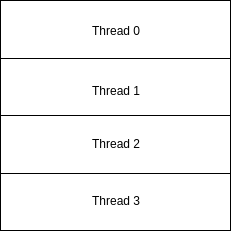
\includegraphics[width=.30\linewidth]{tsplit.png}
  \captionof{figure}{Threads split through the several matrix rows.}
\end{figure}

\par In the previously described example, assuming that $t = 4$, the CSR arrays would be divided into four equal parts. Since the example matrix has 5 rows, one of the threads would compute an extra row. This division is usually responsibility of the OpenMP technology, unless the user specifies the size of chunks to be computed per each thread.

\begin{figure}[!htb]
  \centering
  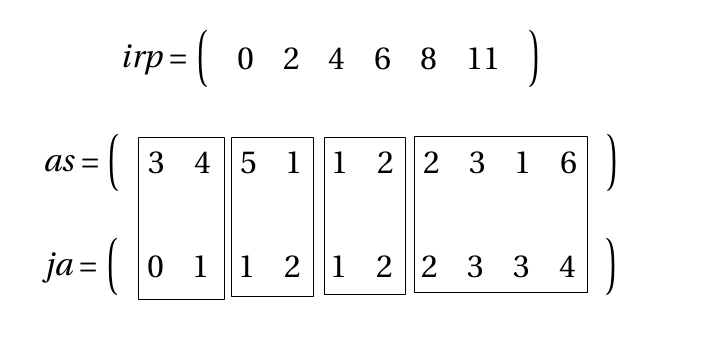
\includegraphics[width=.65\linewidth]{csromp.png}
\end{figure}

\par The Ellpack format would be divided in a similar way.


\begin{figure}[!htb]
  \centering
  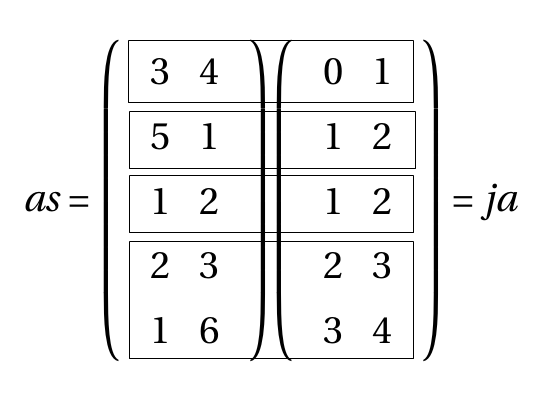
\includegraphics[width=.45\linewidth]{ellomp.png}
\end{figure}

\par The parsing was done with only one thread, therefore some matrix values were already in the reading processor cache memory. Hence, in order to produce "fair" results, the first run was not included in the average of computational times. If it was included, the sequential execution would have a clear advantage on this method. CSR computations could be done with, 

\begin{lstlisting}[style=banner]
int i;
#pragma omp parallel for private(i) schedule(static) num_threads(t)
for (i = 0; i < m; ++i) {
		double temp = 0.0;
		for (int j = irp[i]; j < irp[i + 1]; ++j) {
				temp += as[j] * x[ja[j]];
		}
		y[i] = temp;
}
\end{lstlisting}

and taking the same approach, one could compute matrices in the Ellpack format with, 

\begin{lstlisting}[style=banner]
int i;
#pragma omp parallel for private(i) schedule(static) num_threads(t)
for (i = 0; i < m; ++i) {
		double temp = 0.0;
		for (int j = 0; j < maxnz; ++j) {
				temp += as[i][j] * x[ja[i][j]];
		}
		y[i] = temp;
}
\end{lstlisting}

\par These methods were executed from \textbf{2} to \textbf{16} threads. The method described in this section can be referred as the scalar method.

\subsection*{CUDA}
\addcontentsline{toc}{subsection}{CUDA}

\par The first approach to solve this problem with CUDA was to launch a \textbf{kernel} per row. This method is very similar to the scalar method previously described, and might be the most intuitive and simple solution, but it creates some problems for matrices in the CSR format. Memory access from threads within the same \textit{warp} is not coalesced, thus, like explained before, it is expected that this will become an overhead. 
\par The following code sample can be used as a CSR scalar approach,

\begin{lstlisting}
__global__ void scalarCSR(int * m, int * irp, int * ja, double * as, double * x, double * y) {
		int i = blockIdx.x * blockDim.x + threadIdx.x;
		if (i < *m) {
				double temp = 0.0;
				for (int j = irp[i]; j < irp[i + 1]; ++j) {
					temp += as[j] * x[ja[j]];
				}
				y[i] = temp;
	}
}


\end{lstlisting}

and the the memory access pattern can be described as follows, where the number in the iterations arrays indicates the row to be accessed, 

\begin{center}
\textit{irp}  =   
$
\begin{pmatrix}
    & 0 & 2 & 4 & 6 & 8 & 11 & \\
\end{pmatrix}
$
\linebreak
\textit{as}  =   
$
\begin{pmatrix}
    & 3 & 4 & 5 & 1 & 1 & 2 & 2 & 3 & 1 & 6 & \\
\end{pmatrix}
$
\linebreak
\textit{ja}  =   
$
\begin{pmatrix}
    & 0 & 1 & 1 & 2 & 1 & 2 & 2 & 3 & 3 & 4 & \\
\end{pmatrix}
$
\linebreak
\linebreak
\textit{Iteration 0}  =   
$
\begin{pmatrix}
    & 0 & \_ & 1 & \_ & 2 & \_ & 3 & \_ & 4 & \_ & \_ & \_ &  \\
\end{pmatrix}
$
\linebreak
\textit{Iteration 1}  =   
$
\begin{pmatrix}
    & \_ & 0 & \_ & 1 & \_ & 2 & \_ & 3 & \_ & 4 & \_ & \_ &  \\
\end{pmatrix}
$
\linebreak
\textit{Iteration 2}  =   
$
\begin{pmatrix}
    & \_ & \_ & \_ & \_ & \_ & \_ & \_ & \_ & \_ & \_ & 4 & \_ & \\
\end{pmatrix}
$
\linebreak
\textit{Iteration 3}  =   
$
\begin{pmatrix}
    & \_ & \_ & \_ & \_ & \_ & \_ & \_ & \_ & \_ & \_ & \_ & 4 & \\
\end{pmatrix}
$
\linebreak
\end{center}

 
\par Thereby, by launching a warp per row, is possible to avoid this situation. This methods was denominated as \textbf{Vector-Strip Mining}. It was created an array as shared memory among threads within the same block. In the end, \textbf{sequential} reduction was done among threads within the same \textbf{warp}, reducing the value to the first warp thread. The following piece of code would be an implementation of such strategy \cite{scalar-vm},

\begin{lstlisting}
__global__ void vectorMiningCSR(int * m, int * irp, int * ja, double * as, double * x, double * y) {
	extern __shared__ volatile double sdata[];
	
	int i = blockIdx.x * blockDim.x + threadIdx.x;;
	int warp = i / 32; 
	int lane = i & (32 - 1); 
	int row = warp;

	sdata[threadIdx.x] = 0;

	if (row < *m) {
			for (int j = irp[row] + lane ; j < irp[row + 1]; j += warp_size)
					sdata[threadIdx.x] += as[j] * x[ja[j]];

			if (lane < 16) { sdata[threadIdx.x] += sdata[threadIdx.x + 16]; }
			if (lane < 8) { sdata[threadIdx.x] += sdata[threadIdx.x + 8]; }
			if (lane < 4) { sdata[threadIdx.x] += sdata[threadIdx.x + 4]; }
			if (lane < 2) { sdata[threadIdx.x] += sdata[threadIdx.x + 2]; }
			if (lane < 1) { sdata[threadIdx.x] += sdata[threadIdx.x + 1]; }

			if (lane == 0)
				y[row] += sdata[tid];
	}
}
\end{lstlisting}

\par The memory access pattern is described as follows, 

\begin{center}
\textit{irp}  =   
$
\begin{pmatrix}
    & 0 & 2 & 4 & 6 & 8 & 11 & \\
\end{pmatrix}
$
\linebreak
\textit{as}  =   
$
\begin{pmatrix}
    & 3 & 4 & 5 & 1 & 1 & 2 & 2 & 3 & 1 & 6 & \\
\end{pmatrix}
$
\linebreak
\textit{ja}  =   
$
\begin{pmatrix}
    & 0 & 1 & 1 & 2 & 1 & 2 & 2 & 3 & 3 & 4 & \\
\end{pmatrix}
$
\linebreak
\linebreak
\textit{Iteration 0}  =   
$
\begin{pmatrix}
    & 0 & 0 & \_ & \_ & \_ & \_ & \_ & \_ & \_ & \_ & \_ & \_ &  \\
\end{pmatrix}
$
\linebreak
\textit{Iteration 1}  =   
$
\begin{pmatrix}
    & \_ & \_ & 1 & 1 & \_ & \_ & \_ & \_ & \_ & \_ & \_ & \_ &  \\
\end{pmatrix}
$
\linebreak
\textit{Iteration 2}  =   
$
\begin{pmatrix}
    & \_ & \_ & \_ & \_ & 2 & 2 & \_ & \_ & \_ & \_ & \_ & \_ &  \\
\end{pmatrix}
$
\linebreak
\textit{Iteration 3}  =   
$
\begin{pmatrix}
    & \_ & \_ & \_ & \_ & \_ & \_ & 3 & 3 & \_ & \_ & \_ & \_ & \\
\end{pmatrix}
$
\linebreak
\textit{Iteration 4}  =   
$
\begin{pmatrix}
    & \_ & \_ & \_ & \_ & \_ & \_ & \_ & \_ & 4 & 4 & 4 & 4 & \\
\end{pmatrix}
$
\linebreak
\end{center}

\par In this approach is essential that each warp computes only one row, and it will produce better results if the minimum number of \textit{non-zero} values per row is greater than 32. If so, it will minimize the number of threads idling during the execution of such kernel. With the scalar kernel avoiding this problem becomes more complicated, but it would be minimized if a matrix had the same number of non-zero values per row.
\par The strategy to solve the Sparse Matrix-Vector product when dealing with matrices stored in the Ellpack format was a scalar approach. One kernel per row was launched. Notice that this format has a major drawback of having to perform multiplications by \textit{zero}. 


\section*{Results \& Discussion}
\addcontentsline{toc}{section}{Results \& Discussion}

\par Analysing the produced results was not trivial. One can consider several metrics in order to obtain a proper analysis. As referred before, two main metrics were used. The calculated value of \textit{FLOPS} and the \textit{average non-zero deviation} per row. One should keep in mind that memory may have a big impact in the calculations of this specific problem. The size of \textit{Sparse Matrices} representations in memory may get to \textbf{GigaBytes}, therefore the procedure may achieve a high number of transactions between the several memory levels. Memory transactions are quite expensive, and they should be avoided.

\subsection*{CSR \& Ellpack}
\addcontentsline{toc}{subsection}{CSR \& Ellpack}

\par By taking OpenMP as an example, it could be seen that by having matrices with a very attenuated number of non-zero values per row, the performance of both formats could increase at a similar ratio when the number of threads was increased.

\begin{figure}[!htb]
\centering
\begin{minipage}{.5\textwidth}
  \centering
  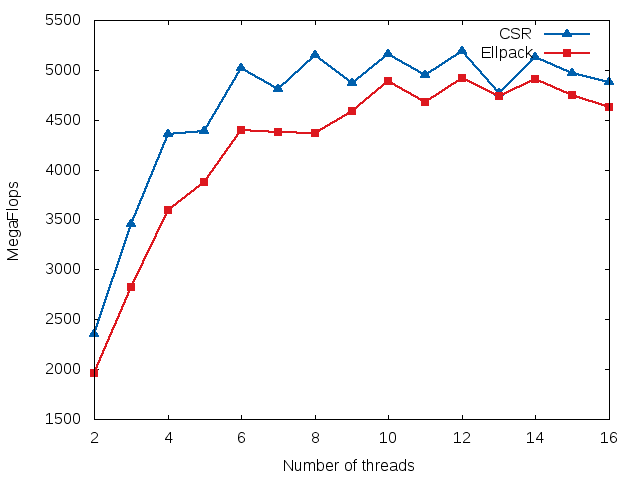
\includegraphics[width=.8\linewidth]{OMP_ML_Laplace.png}
  \captionof{figure}{ML\_ Laplace (1.45\% of nz deviation).}
\end{minipage}%
\begin{minipage}{.5\textwidth}
  \centering
  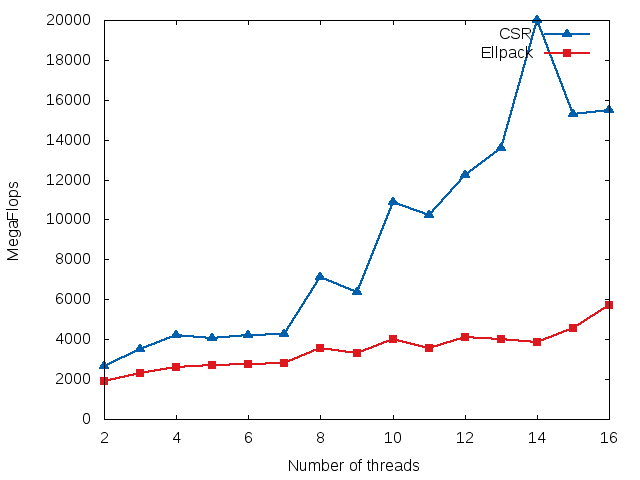
\includegraphics[width=.8\linewidth]{OMP_cant.png}
  \captionof{figure}{cant (20.2\% of nz deviation).}
\end{minipage}
\end{figure}

By observing \textbf{figure 2}, it is possible to observe that this phenomenon occurs with matrix \textit{ML\_ Laplace}, a matrix with $1.45 $\% of average non-zero deviation. But by analysing \textbf{figure 3}, one can determine that such behaviour is not true for matrices with a larger value of \textit{average non-zero deviation} per row. One example of this scenario is matrix \textit{cant}, with $20.2$ \% of this value.

\begin{figure}[!htb]
\centering
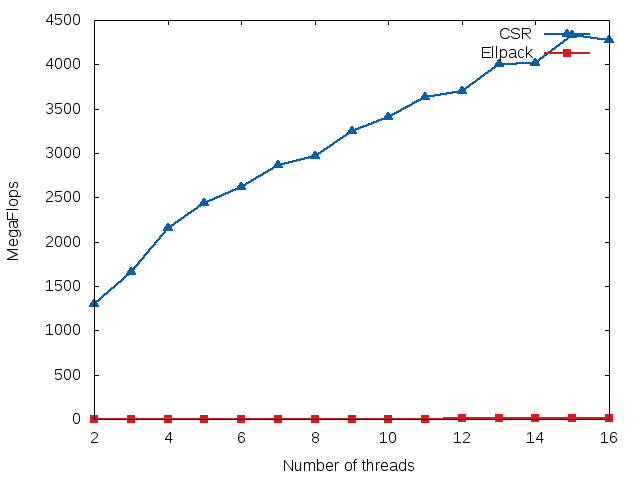
\includegraphics[width=.5\linewidth]{OMP_1M.png}
\captionof{figure}{1M (60.12\% of nz deviation).}
\end{figure}

\par This behaviour is even more radical when dealing with matrices with a higher deviation. The matrix which results can be seen at \textbf{figure 4}, not only has a high deviation of non-zero values per row, but the number of elements to be processed is significantly huge. This is a major overhead for the \textit{Ellpack} format, since multiplications by zero are performed every time a row does not have the maximum number of \textit{non-zero} values.

\subsection*{OpenMP \& CUDA}
\addcontentsline{toc}{subsection}{OpenMP \& CUDA}

\par Parallelization becomes a overhead when one tries to launch threads that will be idle. Such behaviour can be easily seen with small matrices. By analysing \textbf{figure 5}, one can deduce that the number of calculations to be done within this matrix is relatively low. Hence, the performance of parallelization decreases when the number of threads is increased. The overhead of launching threads becomes obvious in these situations. 
\par 
\begin{figure}[!htb]
\centering
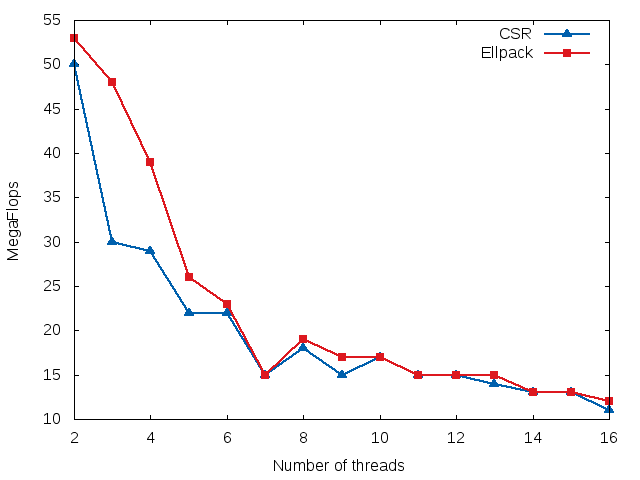
\includegraphics[width=.5\linewidth]{OMP_cage4.png}
\captionof{figure}{OpenMP results of Cage\_ 4, 9 rows, 9 columns, 49 non-zero values.}
\end{figure}

\pagebreak
\section*{Conclusions}
\addcontentsline{toc}{section}{Conclusions}

 

%-------------------------------------------------------------------------------
% REFERENCES
%-------------------------------------------------------------------------------
\newpage
%\addcontentsline{toc}{section}{References}
\begin{thebibliography}{0}

\bibitem{sparse}
Raphael Yuster and Uri Zwick, \textit{Fast sparse matrix multiplication}, Available at: <\url{http://www.cs.tau.ac.il/~zwick/papers/sparse.pdf}> [Accessed 28 March 2018]

\bibitem{sparse-gpu}
B. Neelima1 and Prakash S. Raghavendra, April 2012,  \textit{Effective Sparse Matrix Representation for the
GPU Architectures}, Available at: <\url{https://pdfs.semanticscholar.org/2d15/dd5d0975fff797397ad31059ec097b659e00.pdf}> [Accessed 28 March 2018]

\bibitem{sparse-matrices}
University of Florida, \textit{Sparse Matrix Collection}, Available at: <\url{https://sparse.tamu.edu/}> [Accessed 28 March 2018]

\bibitem{matrix-reader}
Matrix Market, \textit{ANSI C library for Matrix Market I/O}, Available at: <\url{https://math.nist.gov/MatrixMarket/mmio-c.html}> [Accessed 28 March 2018]

\bibitem{cpu-gpu}
B. N. Manjunatha Reddy, Dr. Shanthala S., Dr. B. R. VijayaKuma, February 2017 \textit{Performance Analysis of GPU V/S CPU for Image
Processing Applications}, Available at: <\url{https://www.ijraset.com/fileserve.php?FID=6250}> [Accessed 28 March 2018]


\bibitem{scalar-vm}
Nathan Bell and Michael Garland, December 11, 2008 \textit{Efficient Sparse Matrix-Vector Multiplication on CUDA}, Available at: <\url{http://wnbell.com/media/2008-12-NVR-SpMV/nvr-2008-004.pdf}> [Accessed 8 April 2018]

\bibitem{flame-graphs}
Brendan Greg, \textit{CPU Flame Graphs}, Available at: <\url{http://www.brendangregg.com/FlameGraphs/cpuflamegraphs.html}> [Accessed 9 April 2018]

\end{thebibliography}
\newpage

\section*{Appendices}
\addcontentsline{toc}{section}{Appendices}

\newpage

\subsection*{Project Plan}
\addcontentsline{toc}{subsection}{Project Plan}


\subsection*{Class Diagram}
\addcontentsline{toc}{subsection}{Class Diagram}


\subsection*{Source Code}
\addcontentsline{toc}{subsection}{Source Code}

\end{document}

